% anchor-probe.tex — numerically print circuitikz node-anchor coordinates.
% Use this whenever mos-anchor-cheatsheet.md doesn't already cover a device
% type/transform combo, instead of eyeballing a rendered picture.
%
% Build:  latexmk -pdf -interaction=nonstopmode -halt-on-error anchor-probe.tex
% Read:   pdftotext anchor-probe.pdf -
%
% Edit the \node lines below to add/replace the device+transform combos you
% need to check, then rebuild. Coordinates print in pt, relative to each
% node's own center (so 0,0 = center; sign/axis tells you the anchor side).
\documentclass{standalone}
\usepackage{circuitikz}
\begin{document}
\ctikzset{tripoles/mos style/arrows, transistors/scale=1}
\begin{circuitikz}
  \node[pmos]             (A) at (0,0) {};
  \node[pmos, xscale=-1]  (B) at (0,0) {};
  \node[pmos, yscale=-1]  (C) at (0,0) {};
  \node[pmos, rotate=180] (D) at (0,0) {};
  \node[nmos]             (E) at (0,0) {};
  \node[nmos, xscale=-1]  (F) at (0,0) {};
\end{circuitikz}

\newcommand{\printanchor}[2]{%
  \pgfpointanchor{#1}{#2}%
  \pgfgetlastxy{\myx}{\myy}%
  #1.#2 = (\myx, \myy)\\
}

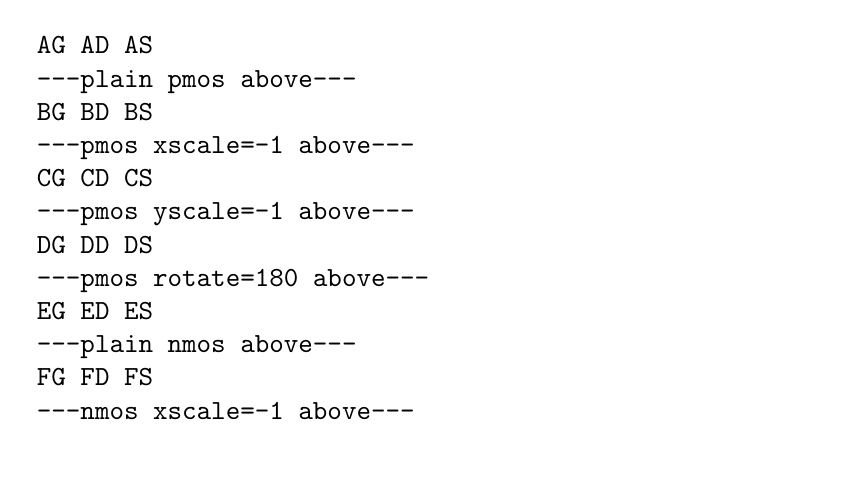
\begin{tikzpicture}
\node{
\begin{minipage}{10cm}
\ttfamily
\printanchor{A}{G} \printanchor{A}{D} \printanchor{A}{S}
\\ ---plain pmos above--- \\
\printanchor{B}{G} \printanchor{B}{D} \printanchor{B}{S}
\\ ---pmos xscale=-1 above--- \\
\printanchor{C}{G} \printanchor{C}{D} \printanchor{C}{S}
\\ ---pmos yscale=-1 above--- \\
\printanchor{D}{G} \printanchor{D}{D} \printanchor{D}{S}
\\ ---pmos rotate=180 above--- \\
\printanchor{E}{G} \printanchor{E}{D} \printanchor{E}{S}
\\ ---plain nmos above--- \\
\printanchor{F}{G} \printanchor{F}{D} \printanchor{F}{S}
\\ ---nmos xscale=-1 above--- \\
\end{minipage}
};
\end{tikzpicture}
\end{document}
